\section{Characterizing the Operational Safety Envelope}
\label{sec:eval}

We design our evaluation to empirically chart the edge-assisted system’s safety envelope under varying latency. Rather than a conventional performance benchmark, our experiments serve as a systematic probe: we first identify the baseline system’s safety breaking point, then demonstrate how our beacon protocol shifts this boundary outward. This section presents our findings in that narrative order.

\subsection{Methodology}
\subsubsection{Experimental Platform}
All experiments were performed using \ecav~\cite{eCAV}, an open-source framework for edge-assisted CAV simulation built upon CARLA~\cite{dosovitskiy_carla_nodate}. CARLA is a high-fidelity simulator built on Unreal Engine 4 that leverages the NVIDIA PhysX engine to model realistic vehicle dynamics. CARLA's physics model is not a simple kinematic model; it is a full physics simulation that accounts for critical real-world factors including engine torque, braking forces, vehicle mass, and tire friction, the latter modeled using the industry-standard Pacejka ``Magic Formula" \cite{pacejka-book}. All agents transmit at a fixed 20\,Hz. The edge publishes at the same tick, yielding an update quantum of 50\,ms.

The use of this high-fidelity physics model is central to our work. It allows us to empirically determine the physical time-to-react boundary (e.g., edge safety envelope) for our scenarios. This boundary is an emergent property of the simulation where the vehicle, subject to realistic physical constraints, can no longer brake or steer in time to avoid a collision. To ensure our results are deterministic and repeatable, we run the CARLA simulator in a synchronous, discrete-time mode with a fixed time step of $\Delta t = 50$~ms on a high-performance workstation (Intel i9-14900k, 192 GB RAM, NVIDIA RTX 4080 Super).

\subsubsection{Scenarios}

To ground our findings in real-world risk, our evaluation focuses on two occlusion-heavy scenarios derived from the official NHTSA Pre-Crash Typology (PCT)~\cite{NHTSA_Typology}:
\begin{enumerate}[label=\arabic*.,noitemsep,topsep=0pt,leftmargin=1.2\parindent]
    \item \textbf{C-Left-Turn-Across-Path/Opposite-Direction (LTAP/OD):} As shown in Fig.~\ref{fig:scenario_left_turn}, an ego vehicle attempts a left turn at an unsignalized intersection while its view of oncoming traffic is obstructed.
    \item \textbf{B-Straight-Crossing-Path (SCP):} As shown in Fig.~\ref{fig:scenario_overtake}, an ego vehicle attempts to overtake a large, stopped vehicle, with its view of a fast-approaching car in the opposite lane being blocked.
\end{enumerate}

\begin{figure}[h]
    \centering
    % Placeholder for the scenario diagram.
    \includegraphics[trim={5cm 5cm 0cm 0cm}, 
        clip,width=\columnwidth]{figures/occluded_left_turn.png}
    \caption{The Occluded Left-Turn Scenario involving two moving vehicles. The ego vehicle (blue) takes a blind left turn, intersecting with the white vehicle's trajectory. The overlaid blue tracks show the chronological progression of the single ego vehicle as it executes the turn. LTAP/OD Pre Crash Typology Code. %\KR{@Tyler: add more text to the caption so that it is clear that what is shown is the track of the ego vehicle in blue doing the left turn.  One could easily mistake there are 5 distinct cars in the picture shown.}
    }
    \label{fig:scenario_left_turn}
\end{figure}


\begin{figure}[h]
    \centering
    % Placeholder for the scenario diagram.
    \includegraphics[width=\columnwidth]{figures/blind_overtake_2.png}
    \caption{The Blind Overtake Scenario. The ego vehicle initiates an overtake of a large stopped vehicle while its view of oncoming traffic (white vehicle) is obstructed. SCP Overtake Pre Crash Typology Code.}
    \label{fig:scenario_overtake}
\end{figure}



\begin{figure}[h]
    \centering
    \includegraphics[width=\columnwidth]{figures/AB3DMOT_scalaiblity.png}
    \caption{Edge tracker scalability. Latency grows quadratically with the number of objects, becoming a significant contributor of the end-to-end pipeline processing time in dense scenarios.}
    \label{fig:scalability}
\end{figure}




\subsubsection{Latency Models}
\label{sec:e2e_lat_model}
To comprehensively characterize the safety envelope, we employ two latency models.

\paragraph{(1) Deterministic latency sweep.}
Our primary experiments use a fixed data-staleness model, in which the total end-to-end latency is a deterministic multiple of the simulation step, i.e., \(L = k \cdot \Delta t\).
This model is useful for isolating the system's core failure mode because it removes randomness in arrival order and lets us sweep latency in controlled increments.

\paragraph{(2) Trace-driven, component-based latency.}
We parameterize a per-step latency model using the component budget in Table~\ref{tab:latency_mec}. At each control tick, the total end-to-end latency is
\[
L \;=\; L_{\mathrm{veh}\rightarrow\mathrm{RSU}} \;+\; L_{\mathrm{backhaul}} \;+\; L_{\mathrm{proc}},
\]
where $L_{\mathrm{veh}\rightarrow\mathrm{RSU}}$ is drawn from SEE-V2X veh$\rightarrow$RSU RTT traces (resampled to $\Delta t$ by nearest-neighbor on emission timestamps), $L_{\mathrm{backhaul}}$ is sampled from a log-normal fit whose median and $p_{99}$ match 5G-MOBIX field trials, and $L_{\mathrm{proc}}$ sums fixed stage latencies measured on our hardware. This parameterization also sizes the reconciliation window $W$ in §\ref{sec:timebase}. We use this model for the jittered results in Fig.~\ref{fig:jitter_results} and for the packet-loss robustness in Table~\ref{tab:loss_sensitivity}.

\subsection{Simulation handling of time and sync}
\label{sec:mapping_sim_to_real}
Our simulator approximates the event-driven design in Section~\ref{sec:timebase} as follows. We run CARLA in synchronous mode with fixed step \(\Delta t=50\,\mathrm{ms}\). Each message carries its generation time (sim time at emission). For deterministic sweeps, the end-to-end latency \(L\) is an integer multiple of \(\Delta t\); for trace-driven runs, \(L\) is the sum of vehicle\(\to\)RSU, RSU\(\to\)edge, and processing components (Section~\ref{sec:e2e_lat_model}). The edge implements a reconciliation window \(W\) and forms frames \([T,\,T{+}W)\) exactly as in the design; \(W\) is chosen to cover the high-percentile jitter of the trace model. The ego planner applies the same use-time admission rule (drop edge objects when \(v_{\text{ego}}\!\cdot\!L \ge r_{\text{gate}}\)). This simulator step-driven time reconciliation preserves the ordering guarantees of GNSS/PTP-disciplined clocks without requiring real hardware clocks in the simulator.



\begin{table}[t]
\footnotesize
\centering
\caption{End-to-end latency components for a MEC deployment (Vehicle→Edge→Vehicle). All stages aligned to a 50 ms control tick.}
\label{tab:latency_mec}
\begin{tabularx}{\columnwidth}{@{}X c@{}}
\toprule
\textbf{Stage} & \textbf{Latency (ms)} \\
\midrule
1. Sensor → On‐board Perception & 20–50 \\
2. Control‐Tick Wait & 0–50 \\
3. Packaging / Serialization & $\sim$5 \\
4. Radio Uplink (C‐V2X PC5 Mode 4)~\cite{Jeon2018ReselectionLookahead} & 30–80 \\
5. Backhaul to MEC Rack~\cite{MECLatency} & $\sim$5~\cite{MECLatency} \\
6. Edge Compute (fusion + tracking + pred) & 20–30 \\
7. Backhaul from MEC~\cite{MECLatency} & $\sim$5~\cite{MECLatency} \\
8. Radio Downlink (C‐V2X PC5 Mode 4)~\cite{Jeon2018ReselectionLookahead} & 30–80~\cite{Jeon2018ReselectionLookahead} \\
9. Control‐Tick Wait & 0–50 \\
10. Planner → Actuation & 5–10 \\
\midrule
\textbf{Total Best‐Case} & $\approx$110 \\
\textbf{Total Average} & $\approx$190 \\
\bottomrule
\end{tabularx}
\vspace{3mm}
\end{table}

\input{floats/tbl-anchoring-packet-loss}



%\begin{figure*}[t]
    \centering
    \subfloat[Occluded Left Turn scenario.]{
    \includegraphics[width=\columnwidth]{figures/olt_false_braking_event.png}
    }
    \subfloat[Blind Overtake scenario.]{
    \includegraphics[width=\columnwidth]{figures/overtake_false_braking_events.png}
    }
    \caption{Efficacy of Self-Beacon Anchoring: False-Braking Events vs. end-to-end latency of the edge-assisted perception pipeline for our two evaluated scenarios. Beacon-Edge: 0 across all latencies. Naive-Edge spikes after ~100 ms.}
    \label{fig:false_braking_results}
\end{figure*}
%\begin{figure*}[t]
    \centering
    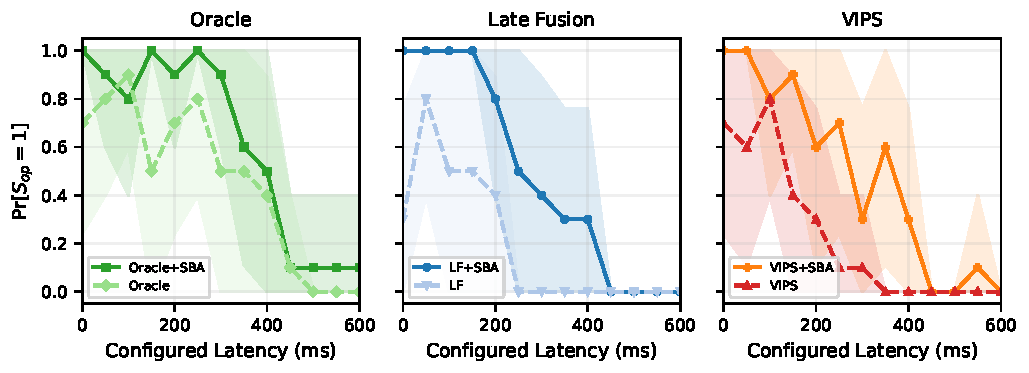
\includegraphics[width=\textwidth]{figures/success_vs_latency.pdf}
    \caption{Operational success $P(S_{op})$ vs.\ configured latency for each manager, with SBA on and off on the same axes. Late Fusion and VIPS exhibit a sharp safety cliff around ${\sim}100\text{--}150\,\mathrm{ms}$. Oracle maintains high $S_{op}$ until the physics-limited boundary at ${\sim}300\text{--}400\,\mathrm{ms}$. With SBA, the multi-source stacks track the Oracle curve.}
    \label{fig:success_vs_latency}
\end{figure*}


%
\begin{figure*}[t]
    \centering
    \subfloat[Occluded Left Turn scenario.]{
    \includegraphics[width=\columnwidth]{figures/olt_ttc_vs_latency.png}
    }
    \subfloat[Blind Overtake scenario.]{
    \includegraphics[width=\columnwidth]{figures/overtake_ttc_vs_latency.png}
    }
    \vspace{-3mm}
    \caption{Average Time-to-Collision (TTC) vs. end-to-end latency of the edge-assisted perception pipeline for our two evaluated scenarios. The Beacon-Edge system consistently provides a larger safety margin (higher TTC) across latencies.}
    \label{fig:ttc_vs_latency}
\end{figure*}

\input{floats/float-combined-success-braking-ttc}



\begin{figure*}[t]
    \centering
\captionsetup[subfigure]{skip=-15pt}
    % --- SUBFIGURE (a) ---
    \begin{subfigure}[b]{0.24\textwidth}
        \centering
        \includegraphics[width=\linewidth]{figures/box_totals.png}
        \caption{Overall Latency Breakdown.}
        \label{fig:box_totals}
    \end{subfigure}\hfill % NO blank line after this
    % --- SUBFIGURE (b) ---
    \begin{subfigure}[b]{0.24\textwidth}
        \centering
        \includegraphics[width=\linewidth]{figures/box_vehicle.png}
        \caption{Vehicle-Side Components.}
        \label{fig:box_vehicle}
    \end{subfigure}\hfill % NO blank line after this
    % --- SUBFIGURE (c) ---
    \begin{subfigure}[b]{0.24\textwidth}
        \centering
        \includegraphics[width=\linewidth]{figures/box_edge.png}
        \caption{Edge-Side Components.}
        \label{fig:box_edge}
    \end{subfigure}\hfill % NO blank line after this
    % --- SUBFIGURE (d) ---
    \begin{subfigure}[b]{0.24\textwidth}
        \centering
        \includegraphics[width=\linewidth]{figures/edge_latency_compare_box.png}
        \caption{Edge Compute Cost.}
        \label{fig:edge_compute_cost}
    \end{subfigure}
    % All subfigures are now on a "single line" in the code.
    %\vspace{-3mm}
    \caption{Processing-time breakdown of the end-to-end perception pipeline. (a) End-to-end latency is dominated by network and on-vehicle processing. (b) On-vehicle, perception (YOLOv5) is the main contributor. (c) On-edge, the tracker (AB3DMOT) is the main contributor. (d) The overhead of our proposed Beacon-Edge protocol is negligible ($\sim$0.2ms).}
    \label{fig:latency_breakdown_combined}
\end{figure*}
\begin{table}[t]
\footnotesize
\centering
\caption{Per-vehicle uplink budget at \textbf{20 Hz}.
         Statistics computed over all frames in both scenarios
         (\(n\!=\!2{,}000\)); each vehicle sent at most 10 boxes per frame.}
\label{tab:bandwidth}
\begin{tabularx}{\linewidth}{@{}lccc@{}}
\toprule
\textbf{Msg type} & \textbf{Avg.\ size (B)} & \textbf{p95 (B)} & \textbf{KB/s}\\
\midrule
Self-beacon (fixed)        & 96   & 96    & 1.88 \\
3-D bbox list ($\leq$10 boxes)  & 4,130 & 4,720 & 8.06 \\
\midrule
\textbf{Total}             & —    & —     & \textbf{9.94} \\
\bottomrule
\end{tabularx}
%\vspace{-0.6em}
\end{table}
%We benchmarked the computational and bandwidth costs to ensure our system is practical. The overhead of our self-beaconing logic is negligible, adding only 0.2~ms of compute time (Fig.~\ref{fig:edge_compute_cost}). The total uplink bandwidth per vehicle is approximately 9.9 KB/s, which is one to two orders of magnitude lower than feature-streaming systems like F-Cooper~\cite{fcooper} or V2X-ViT~\cite{v2xvit2022} (Table~\ref{tab:bandwidth}). These results confirm the efficiency of our approach.

\subsection{System Overhead Quantification}
\label{sec:eval:overhead}

Fig.~\ref{fig:latency_breakdown_combined} breaks down the processing time of our end-to-end pipeline into four views.

\textbf{Overall (Fig.~\ref{fig:box_totals}).}
The total latency per perception-and-fusion cycle is dominated by the vehicle side and the two radio legs.
This result is consistent with our latency budget in Table~\ref{tab:latency_mec}: even in realistic V2X settings, edge compute is not the bottleneck.

\textbf{Vehicle side (Fig.~\ref{fig:box_vehicle}).}
On the vehicle, neural perception (YOLOv5) is by far the largest component.
Serialization and V2X transmission account for a small fraction of the frame time, which justifies our choice of late fusion: we uplink compact object lists and beacons rather than high-dimensional features.

\textbf{Edge side (Fig.~\ref{fig:box_edge}).}
At the edge, the multi-object tracker (AB3DMOT) is the main consumer of compute.
Time reconciliation, beacon lookup, and publication are small constant-time stages.
This separation is important because it lets us attribute failures to state-consistency effects rather than to heavy learned fusion models.

\textbf{Protocol cost (Fig.~\ref{fig:edge_compute_cost}).}
Adding our self-beacon anchoring logic to the edge pipeline increases per-frame latency by only \(\approx 0.2\,\mathrm{ms}\).
In other words, enforcing the Ego-Uniqueness invariant is effectively free compared to the base tracker.

Finally, the per-vehicle uplink required by this configuration is \(\approx 9.9~\mathrm{KB/s}\) (Table~\ref{tab:bandwidth}), which is one to two orders of magnitude lower than feature- or point-cloud–streaming approaches such as F-Cooper~\cite{fcooper} or V2X-ViT~\cite{v2xvit2022}. The results show that the consistency mechanism is compatible with current DSRC/C-V2X link budgets.


\subsection{The Masking Effect of the State-Consistency Cliff}
\label{sec:masking_effect}

We now present the empirical results that validate the central claims. Our first experiment characterizes the safety envelope of a baseline system to test the hypothesis of a ``safety cliff.'' The orange \texttt{Naive-Edge} curve in Figs.~\ref{fig:summary_metrics}\subref{fig:success_vs_latency},\subref{fig:success_vs_latency_overtake} provides quantitative evidence: success remains near 100\% at low latencies, then drops sharply around 100--150\,ms end-to-end latency.

As shown earlier in Fig.~\ref{fig:seq_selfghost}, the naive edge tracker can birth a stale ego track from a late $t_0$ beacon; the subsequent $t_1$ beacon then fails the spatial gate and births a duplicate, which the planner interprets as a distinct obstacle, causing a spurious brake.

To identify the root cause in aggregate, Figs.~\ref{fig:summary_metrics}\subref{fig:false_braking_results},\subref{fig:false_braking_results_overtake} plots hazardous braking events versus latency. The orange \texttt{Naive-Edge} curve exhibits a sharp increase that aligns with the success cliff in Figs.~\ref{fig:summary_metrics}\subref{fig:success_vs_latency},\subref{fig:success_vs_latency_overtake}. This alignment shows that the observed boundary is logic-induced (state-consistency failure), not physics-induced. The effect masks behavior at higher latencies, preventing characterization of the true physical limit. We therefore enable the anchoring protocol in Section~\ref{sec:unmasking} to remove this masking and expose the physical boundary.

\input{floats/float-olt-jitter}

\noindent\textbf{Trace-driven validation.}
We repeated the same LTAP/OD experiment using the trace-driven latency model from Sec.~\ref{sec:e2e_lat_model}.
Fig.~\ref{fig:jitter_results} shows that the \texttt{Naive-Edge} system exhibits an almost identical safety cliff under realistic C-V2X and backhaul jitter: success stays near 100\% at low realized latency, then collapses once several samples exceed \(\approx 150\,\mathrm{ms}\). We confirm that the masking effect is not an artifact of the deterministic sweep, but a consequence of a latency-induced consistency failure that also manifests under real traces.

\noindent\textbf{Packet-loss robustness.}
We stress the trace-driven model with per-message Bernoulli losses and short bursts. Table~\ref{tab:loss_sensitivity} reports hazardous brakes, scenario success, and TTC under increasing loss. Anchoring preserves a single ego track across outages up to $\texttt{MAX\_AGE}_B$ frames (no duplicate births), maintaining success while the Naive-Edge baseline exhibits residual false brakes and degraded recall.


%This \KR{@Tyler: dangling this} demonstrates that in the baseline system, the operational safety envelope is strictly bounded by this logic-based state-consistency failure.

\subsection{Unmasking the Envelope with Self-Beacon Anchoring}
\label{sec:unmasking}

Having established the state-consistency cliff as the primary, masking boundary, we now apply our self-beacon anchoring protocol. The goal of this experimental phase is to demonstrate that by resolving this specific logic-based failure, we can stabilize the system and enable a more complete characterization of the safety envelope at higher latencies.

The direct evidence of the protocol's efficacy is shown in Figs.~\ref{fig:summary_metrics}\subref{fig:false_braking_results},\subref{fig:false_braking_results_overtake}. The blue \texttt{Beacon-Edge} curve shows zero false-braking events across all tested latencies versus a dramatic spike for the orange \texttt{Naive-Edge} beyond 100ms latency. This result confirms that our protocol, by enforcing the Ego-Uniqueness Invariant at the edge tracker, completely and deterministically eliminates the ``self-ghost\-ing'' failure mode.

The impact of this fix on the end-to-end safety outcome is shown in Figs.~\ref{fig:summary_metrics}\subref{fig:success_vs_latency},\subref{fig:success_vs_latency_overtake}. By eliminating the hazardous braking events, our \texttt{Beacon-Edge} protocol restores the Scenario Success Rate to 100\% in the 150-300~ms latency range where the baseline system's performance had collapsed. In other words, by fixing the consistency logic, we double the safe latency threshold from ~100ms to around 200–250ms (and in some trials up to 300 ms) – substantially expanding the edge-assisted safety envelope

Furthermore, our protocol not only increases the success rate but also improves the qualitative safety margin of those successes. As shown in Figs.~\ref{fig:summary_metrics}\subref{fig:ttc_vs_latency},\subref{fig:ttc_vs_latency_overtake}, the \texttt{Beacon-Edge} system consistently maintains a higher and more stable Average Time-to-Collision (TTC) compared to the baseline. Our results indicate that even in non-failure scenarios, our protocol provides the vehicle with a larger buffer for safe decision-making. Under loss, the same trend holds: Table~\ref{tab:loss_sensitivity} shows that anchoring sustains success and eliminates false brakes across the tested loss rates, whereas Naive-Edge degrades as loss increases.


With the logic-based failure resolved and the system's stability confirmed across multiple metrics, we can now operate safely at latencies that were previously inaccessible. This resolution permits us to proceed with the final phase of our investigation: characterizing the true physical boundaries of the architecture. 

\subsection{Discovering the True Physical Safety Boundary}
\label{sec:physical_boundary}

Eliminating self-ghosting enables a direct test of our second hypothesis from the introduction: the latency threshold imposed by a logic-induced consistency failure is substantially lower than the true physical time-to-react limit.
In the deterministic sweep (Figs.~\ref{fig:summary_metrics}\subref{fig:success_vs_latency},\subref{fig:success_vs_latency_overtake}), enabling the protocol shifts first failures to approximately 300--400~ms of end-to-end latency. We observe the same transition in the trace-driven experiments (Fig.~\ref{fig:jitter_results}), although with wider variance because several SEE-V2X/5G-MOBIX samples cluster high-latency events back-to-back. In both cases, these results confirm that the dominant safety boundary in the baseline configuration arises from a state-consistency failure rather than from the vehicle’s braking dynamics. By co-designing the edge pipeline to enforce identity consistency, we move the observed failure point out to the physics-bound regime and expand the safe operating envelope by more than 2\(\times\).

As a synthesis of these findings, Table~\ref{tab:summary-envelope} contrasts the dominant failure mode and resulting latency cliff across configurations.
\input{floats/tbl-summary}


With the protocol enabled, success remains near 100\% until roughly 300–400~ms, after which the success rate declines sharply. Post-hoc analysis of these runs shows that the remaining failures are no longer attributable to self-ghosting. Instead, they reflect physical-limit cases in which, despite perfectly consistent state estimates, the planner cannot synthesize an avoidance trajectory in time given the simulated constraints on braking and steering.

These results identify the \textbf{true physical boundary} of the operational safety envelope for this scenario. They also demonstrate a key scientific finding: the primary safety boundary observed in the baseline system is due to a logic-level consistency fault. Only after enforcing state consistency through the proposed protocol could we empirically expose the system’s physical limit and quantify the resulting 2× expansion of the safe operating region.


